%!TEX TS-program = xelatex
%!TEX encoding = UTF-8 Unicode
% Awesome CV LaTeX Template for Cover Letter
%
% This template has been downloaded from:
% https://github.com/posquit0/Awesome-CV
%
% Authors:
% Claud D. Park <posquit0.bj@gmail.com>
% Lars Richter <mail@ayeks.de>
%
% Template license:
% CC BY-SA 4.0 (https://creativecommons.org/licenses/by-sa/4.0/)
%


%-------------------------------------------------------------------------------
% CONFIGURATIONS
%-------------------------------------------------------------------------------
\def\COLOR{00008b}
\def\HIGHLIGHT_TITLES{false}

% A4 paper size by default, use 'letterpaper' for US letter
\documentclass[11pt, a4paper]{awesome-cv}

% Configure page margins with geometry
\geometry{left=1.4cm, top=.8cm, right=1.4cm, bottom=1.8cm, footskip=.5cm}

% Specify the location of the included fonts
\fontdir[fonts/]

% Color for highlights
\definecolor{awesome}{HTML}{\COLOR}

% Colors for text
% Uncomment if you would like to specify your own color
% \definecolor{darktext}{HTML}{414141}
% \definecolor{text}{HTML}{333333}
% \definecolor{graytext}{HTML}{5D5D5D}
% \definecolor{lighttext}{HTML}{999999}

% Set false if you don't want to highlight section with awesome color
\setbool{acvSectionColorHighlight}{\HIGHLIGHT_TITLES}

% If you would like to change the social information separator from a pipe (|) to something else
\renewcommand{\acvHeaderSocialSep}{\quad\textbar\quad}


%-------------------------------------------------------------------------------
%	PERSONAL INFORMATION
%	Comment any of the lines below if they are not required
%-------------------------------------------------------------------------------
\def\FIRST_NAME{Gurdeep}
\def\LAST_NAME{Kumar}
\def\POSITION{Network Operations Engineer}
\def\ADRESS{}
\def\MOBILE{(+41) 0779932804}
\def\EMAIL{gurdipku91@gmail.com}
\def\GITHUB{hnnthecore}
\def\LINKEDIN{hnnthecore}
\def\HOMEPAGE{itswisskumar.ch}
\def\GITLAB{}
\def\SO_ID{}
\def\SO_NAME{}
\def\TWITTER{}
\def\SKYPE{}
\def\REDDIT_ID{}
\def\MEDIUM_ID{}
\def\GOOGLE_SCHOLAR_ID{}
\def\GOOGLE_SCHOLAR_NAME{}
\def\EXTRA_INFO{}
%\def\QUOTE{``You can' t judge a book by its cover"}
\def\QUOTE{``Quality is never an accident; it is always the result of intelligent effort."}
% Available options: circle|rectangle,edge/noedge,left/right

%\photo[right,rectangle,noedge]{./photo/photo.jpg}
\name{\FIRST_NAME}{\LAST_NAME}
\position{\POSITION}
%\address{\ADRESS}
\mobile{\MOBILE}
\email{\EMAIL}
\github{\GITHUB}
\linkedin{\LINKEDIN}
%\homepage{\HOMEPAGE}
% \gitlab{\GITLAB}
% \stackoverflow{\SO_ID}{\SO_NAME}
% \twitter{\TWITTER}
% \skype{\SKYPE}
% \reddit{\REDDIT_ID}
% \medium{\MEDIUM_ID}
% \googlescholar{\GOOGLE_SCHOLAR_ID}{\GOOGLE_SCHOLAR_NAME}
% \extrainfo{\EXTRA_INFO}

\quote{\QUOTE}


%-------------------------------------------------------------------------------
%	LETTER INFORMATION
%	All of the below lines must be filled out
%-------------------------------------------------------------------------------
% The company being applied to
\recipient
  {Swisscom}
  {Alte Tiefenaustrasse 6\\
  3048 Ittigen\\}
% The date on the letter, default is the date of compilation
\letterdate{\today}
% The title of the letter
\lettertitle{Bewerbung als Network Operations Engineer}
% How the letter is opened
\letteropening{}
% How the letter is closed
\letterclosing{Freundliche Grüsse,}
% Any enclosures with the letter
%\letterenclosure[Attached]{Curriculum Vitae}


%-------------------------------------------------------------------------------
\begin{document}

% Print the header with above personal informations
% Give optional argument to change alignment(C: center, L: left, R: right)
\makecvheader[R]

% Print the footer with 3 arguments(<left>, <center>, <right>)
% Leave any of these blank if they are not needed
\makecvfooter
  {\today}
  {\FIRST_NAME \LAST_NAME~~~·~~~Motivationsschreiben}
  {}

% Print the title with above letter informations
\makelettertitle

%-------------------------------------------------------------------------------
%	LETTER CONTENT
%-------------------------------------------------------------------------------
\begin{cvletter}
	

\lettersection{Über mich}

Ich bin eine entschlossene und detailorientierte Person, die stets nach Präzision in allem strebt, was ich tue. Meine Leidenschaft für Technologie motiviert mich dazu, unzählige Stunden mit dem Studium, der Recherche und dem Erkunden neuer Technologien zu verbringen, um meine Neugier zu befriedigen. Ich habe ein tiefes Interesse daran, zu verstehen, wie Dinge funktionieren, was meine Liebe zum Problemlösen und zur Innovation antreibt. Ich tauche gerne in komplexe Herausforderungen ein, sei es beim Programmieren, im Systemdesign oder beim Erlernen neuer Technologien.

Meine Entschlossenheit treibt mich nicht nur dazu an, Neues zu lernen, sondern die Themen, die mich interessieren, auch zu meistern. Ich bin fest davon überzeugt, dass lebenslanges Lernen der Schlüssel ist, und ich achte bewusst darauf, stets auf dem neuesten Stand der Trends in der Technologiebranche zu bleiben. Diese Einstellung hilft mir, anpassungsfähig zu bleiben und sowohl persönlich als auch beruflich kontinuierlich zu wachsen. Ich schätze die Zusammenarbeit mit Kollegen, um Ideen auszutauschen und gemeinsame Ziele zu erreichen. Mein Ziel ist es, meine technischen Fähigkeiten mit meiner Leidenschaft für Kreativität zu kombinieren, um an innovativen und bedeutsamen Projekten mitzuwirken.


\lettersection{Was qualifiziert mich als Network Operations Engineer?}
In den letzten Jahren habe ich mich intensiv mit Netzwerktechnik beschäftigt und grundlegende Kenntnisse über Protokolle wie TCP/IP, BGP, OSPF und HSRP aufgebaut. Dabei habe ich ein gutes Verständnis für die Funktionsweise von Switching auf Layer 2 und Layer 3 erlangt.

Um meine Kenntnisse praktisch anzuwenden und zu vertiefen, baue ich aktuell mein eigenes Netzwerk-Labor mit physischer Hardware auf. Obwohl ich bereits praktische Erfahrung mit Netzwerksimulationen in **Cisco Packet Tracer und GNS3** gesammelt habe, war es mir wichtig, auch mit echter Hardware zu arbeiten. Dies ermöglicht es mir, nicht nur die theoretischen Konzepte besser zu verstehen, sondern auch reale Konfigurationen durchzuführen und praxisnah zu experimentieren.

Aktuell bereite ich mich auf die **SIZ-Zertifizierung** vor, für die ich in den nächsten Monaten meine Prüfungen ablegen werde. Da ich bereits intensiv für die **CCNA-Zertifizierung von Cisco** gelernt habe, aber die Prüfung verschoben habe, um genügend Zeit für die Vorbereitung auf die SIZ-Zertifizierung zu haben, plane ich, nach deren Abschluss das CCNA-Studium wieder intensiv aufzunehmen. Mein Ziel ist es, beide Zertifizierungen erfolgreich zu absolvieren.


Auch wenn ich noch keine umfangreiche Praxiserfahrung habe, bringe ich eine grosse Lernbereitschaft, Leidenschaft für Netzwerktechnologien und den Willen mit, mich kontinuierlich weiterzuentwickeln. 


\newpage % Nuova pagina

\lettersection{Mein Homelab}

\begin{figure}[h!]
    \centering
    \begin{minipage}{0.48\textwidth} % Prima immagine
        \centering
        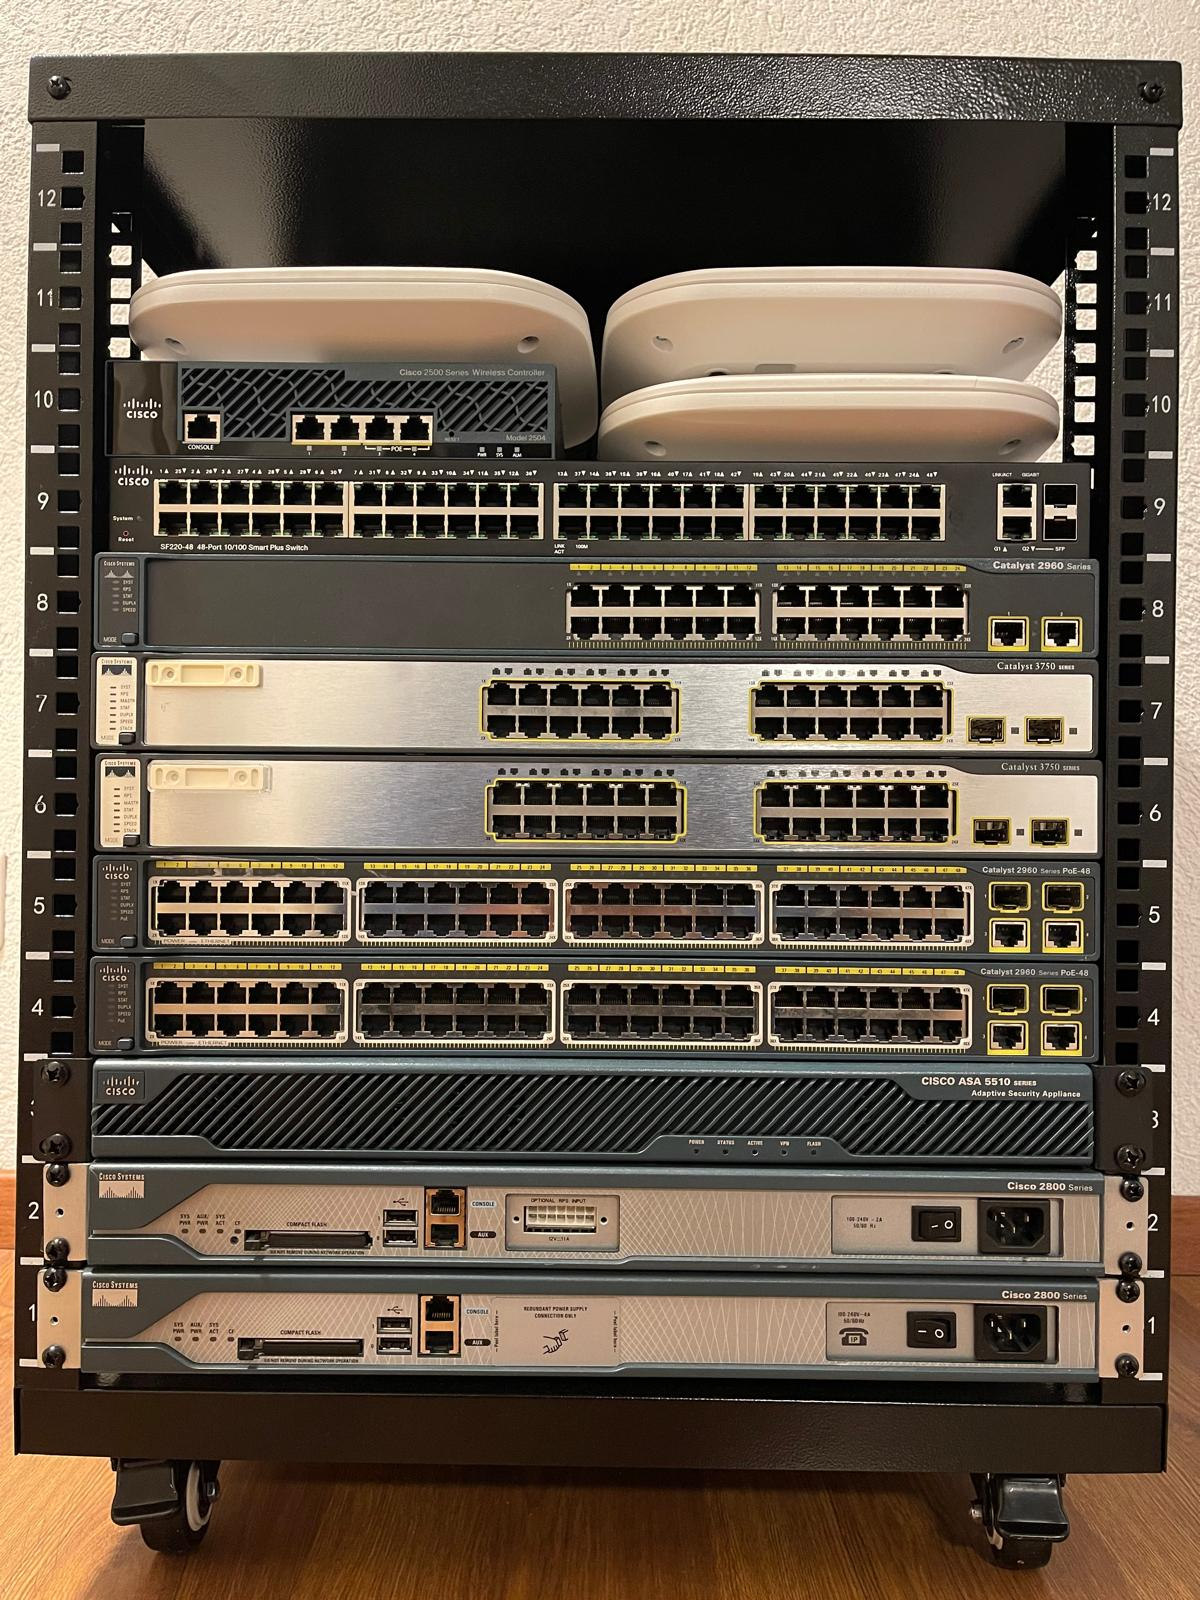
\includegraphics[width=\textwidth]{./foto_lab/lab_1.jpg}
        \caption{Cisco Router und Switches}
        \label{fig:lab1}
    \end{minipage}
    \hfill
    \begin{minipage}{0.48\textwidth} % Seconda immagine
        \centering
        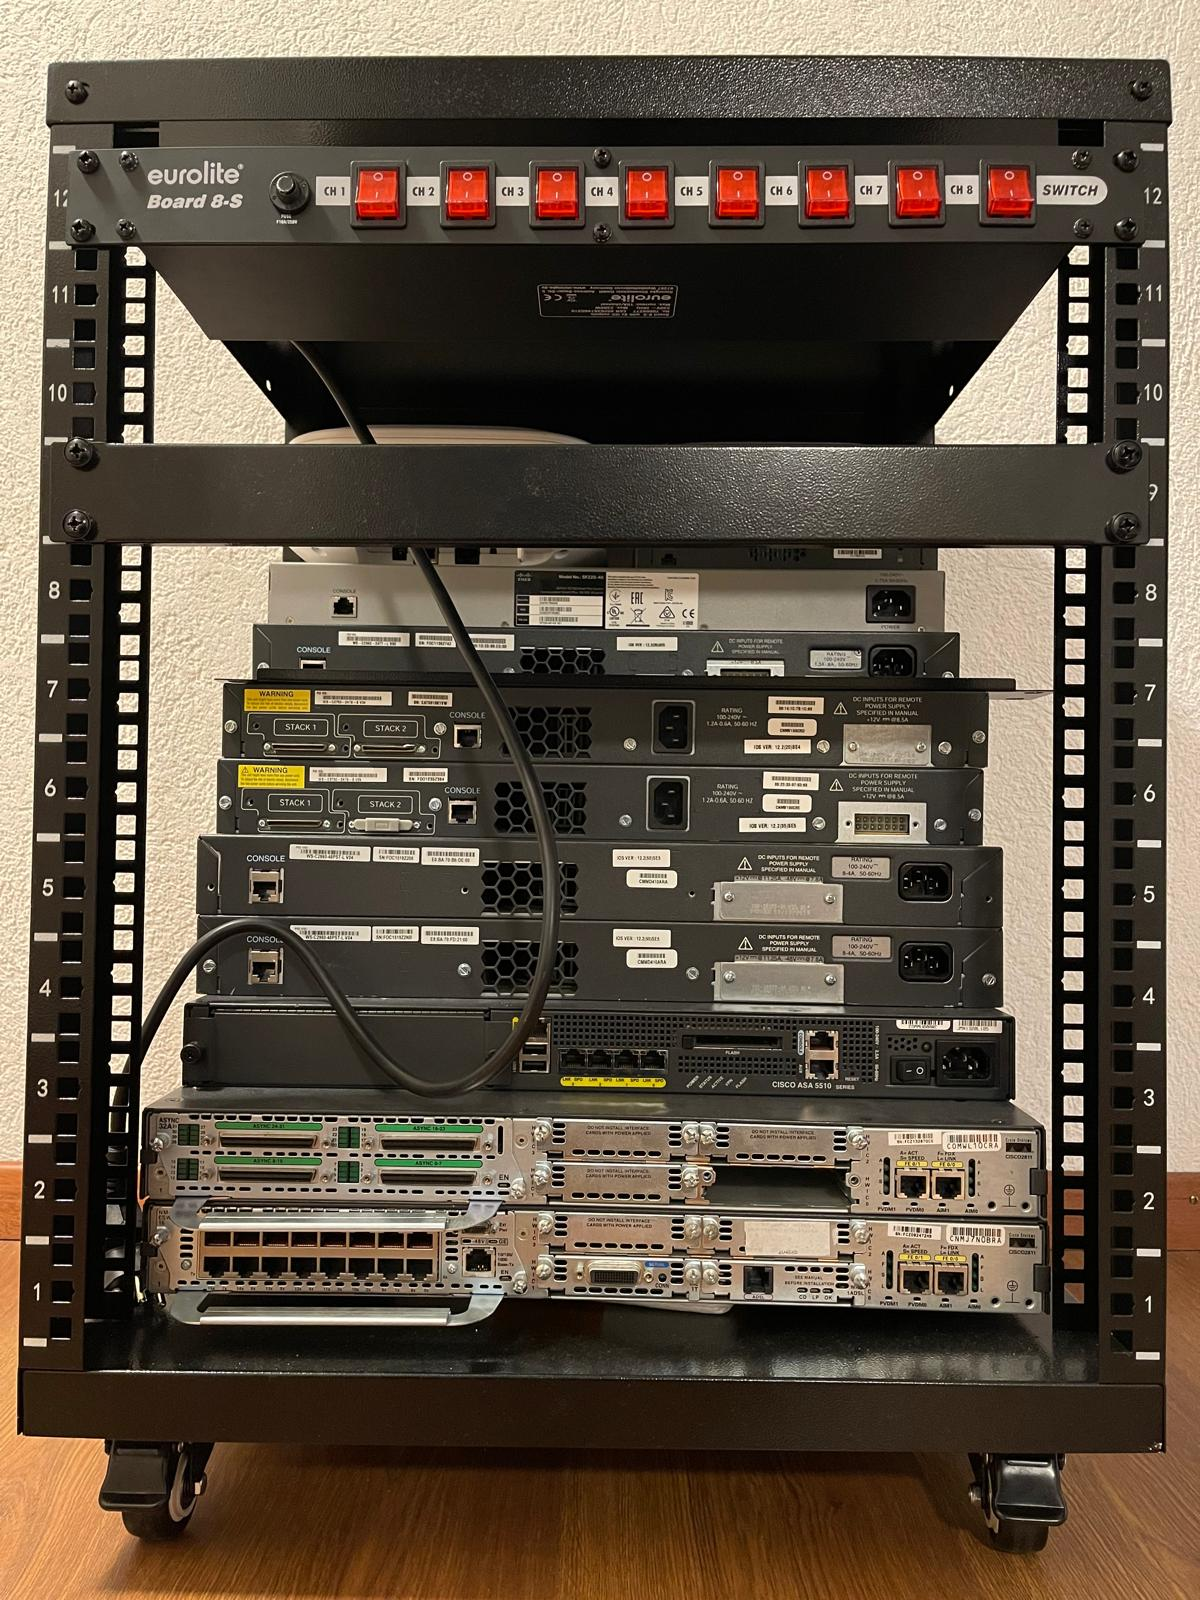
\includegraphics[width=\textwidth]{./foto_lab/lab3.jpg}
        \caption{Netzwerk-Geräte in Aktion}
        \label{fig:lab2}
    \end{minipage}
\end{figure}

\vspace{0.5cm}


Mein persönliches Homelab besteht aus einer Vielzahl von Netzwerkgeräten, die mir helfen, reale Netzwerktopologien zu simulieren und verschiedene Protokolle zu testen. Dies ermöglicht mir, meine praktischen Fähigkeiten kontinuierlich zu verbessern und ein tiefes Verständnis für Netzwerktechnologien zu entwickeln.

\textbf{In meinem Homelab befinden sich folgende Geräte:}
\begin{itemize}
    \item 2x Cisco 2800 Router
    \item 1x Cisco ASA 5510 Firewall
    \item 2x Cisco Catalyst 2960 Layer-2 Switches
    \item 2x Cisco Catalyst 3750 Layer-3 Switches
    \item 1x Cisco WLC 2500 Wireless Controller
    \item 3x Cisco Access Points
\end{itemize}


Diese Geräte ermöglichen es mir, verschiedene Netzwerkarchitekturen zu konfigurieren, Routing- und Switching-Techniken zu testen sowie Sicherheitslösungen mit Firewalls und drahtlosen Netzwerken zu implementieren.




\end{cvletter}


%-------------------------------------------------------------------------------
% Print the signature and enclosures with above letter informations
\makeletterclosing

\end{document}
